\begin{frame}{Preplanned Bike Extensions}
	\begin{mycolumns}[columns=4,T]
		\centering\pic[width=\linewidth]{bike-extensionpoint1}

		bike lock
	\mynextcolumn
		\centering\pic[width=\linewidth]{bike-extensionpoint2}

		front wheel brake
	\mynextcolumn
		\centering\pic[width=\linewidth]{bike-extensionpoint3}

		rear wheel brake
	\mynextcolumn
		\centering\pic[width=\linewidth]{bike-extensionpoint4}

		kickstand
	\end{mycolumns}
\end{frame}

\begin{frame}{Preplanned Bike Extensions}
	\begin{mycolumns}[columns=5,widths={30,5,30,5,30}]
		\centering\pic[width=\linewidth]{bike-extensionpoint1-withoutplugin}

		framework with extension~points
	\mynextcolumn
		\centering\Huge +
	\mynextcolumn
		\centering\pic[width=\linewidth]{bike-lock}

		plug-ins\\~
	\mynextcolumn
		\centering\Huge =
	\mynextcolumn
		\centering\pic[width=\linewidth]{bike-extensionpoint1}

		framework with plug-ins\\~
	\end{mycolumns}
\end{frame}

\subsection{Frameworks with Plug-Ins}
\begin{frame}{\myframetitle\ \mytitlesource{\featureide}}
	\leftorright{
		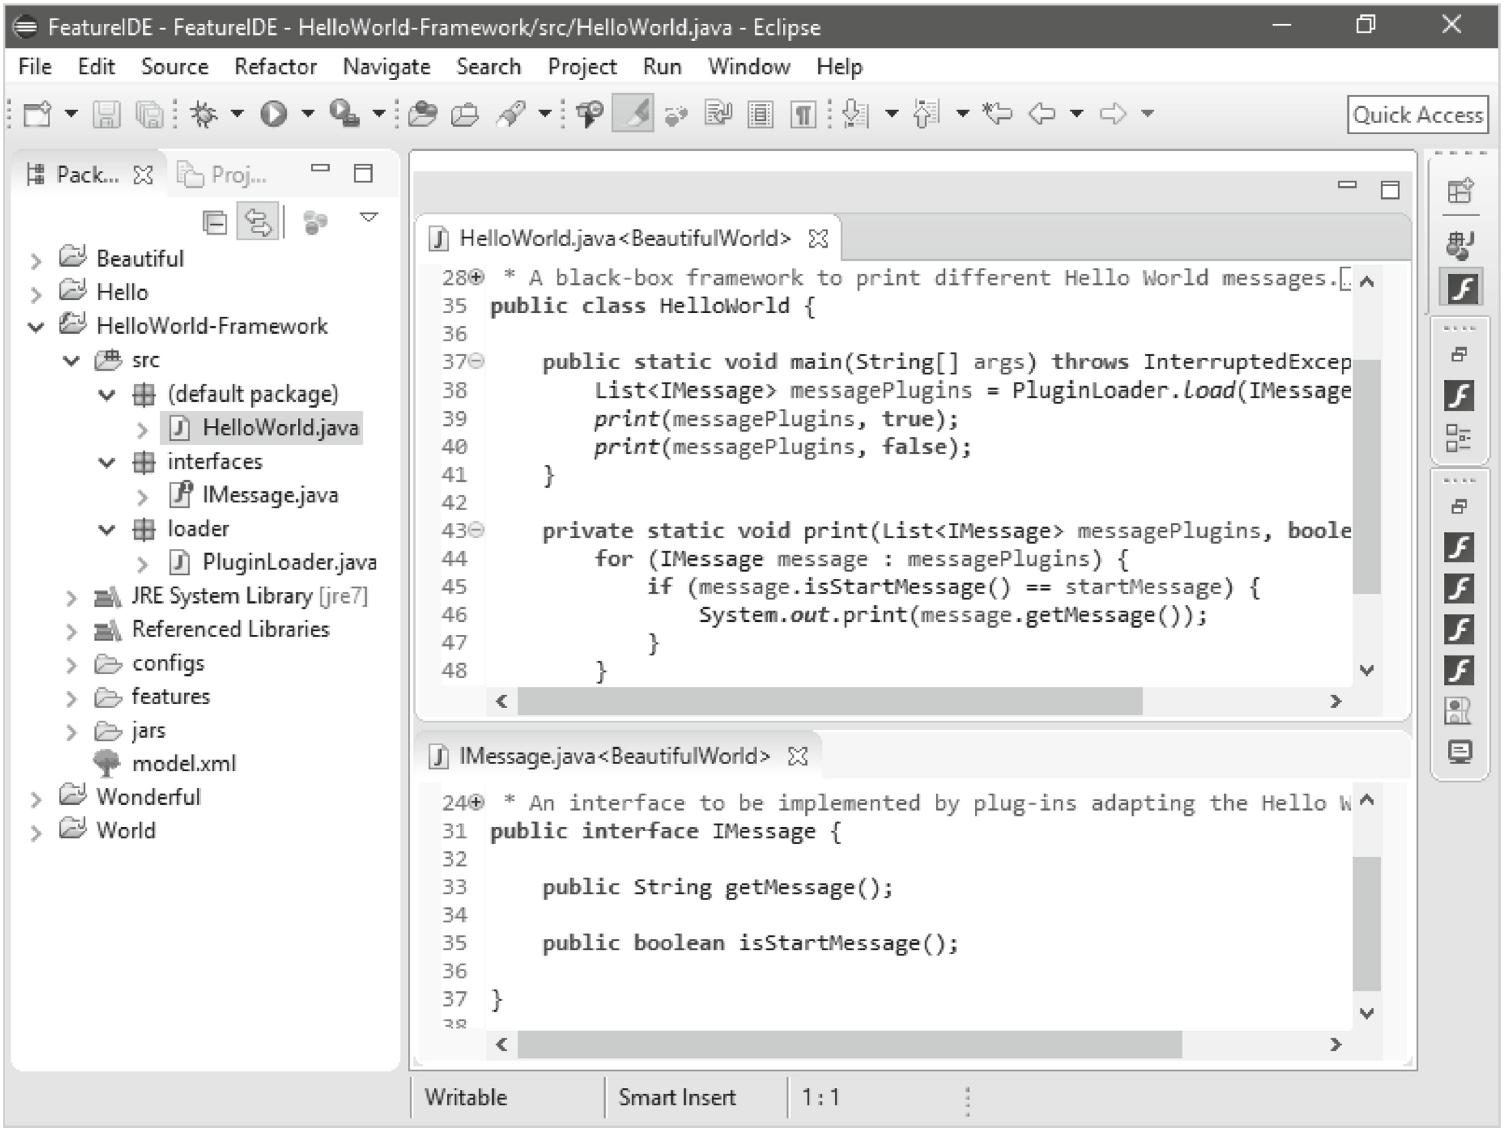
\includegraphics[width=\linewidth]{framework-with-plugins}
	}{
		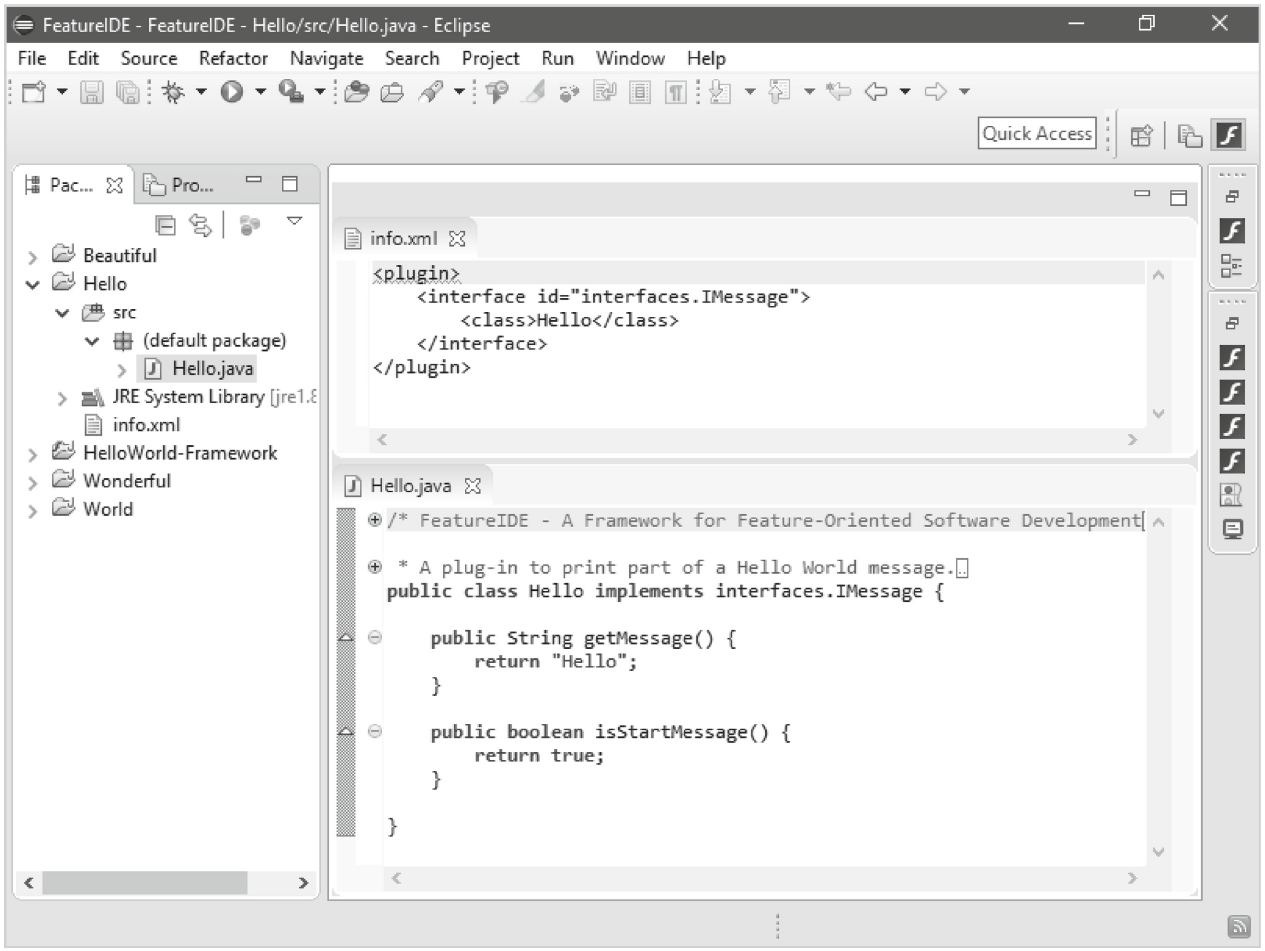
\includegraphics[width=\linewidth]{framework-a-plugin}
	}
\end{frame}

\subsection{White-Box Frameworks?}
% discuss differences to black-box and similiarities to components with gluecode

